\chapter{Investigations of the Equations of Motion}\label{chap2}

\begin{enumerate}
	\item (16) Show that through every phase point there is one and only one	phase curve.\par 
	Solution: The phase flow is given by the equations
	\begin{equation}\label{flow}
		\dot{x} = y\hspace{1cm} \dot{y} = f(x).
	\end{equation}
	The equation for $y$ can be written as
	\begin{align}
		\diff{y}{x} y &= f(x)\\
		\implies \int_{y_0}^{y} y'\mathrm{d}y' & = \int_{x_0}^x f(x')\mathrm{d}x\\
		\implies \frac{y^2}{2} - F(x) &= \frac{y_0^2}{2} - F(x_0) = const.\label{eqflow}
	\end{align}
where $(x_0,y_0)$ are initial conditions, and $F(x)$ is the anti-derivative of $f(x)$, which is defined up to a constant. We note that due to the appearance of $F$ on both sides of equation \eqref{eqflow}, the choice of this arbitrary constant is not important. The equation \eqref{eqflow} is the equation of a 1-D curve in phase space that passes through the point $(x_0,y_0)$. This is a well defined unique curve that is determined by only the initial conditions, which can be taken at any point on the curve. \qed
\item (18) Prove this (that the local maximum points ofthe
potential energy are unstable, but the minimum points are stable equilibrium
positions).\par
Problem: The solution to this is straightforward. $f(x) = -\mathrm{d}U/\mathrm{d}x = U'(x)$, where $U$ is the potential. If $x_0$ is an equilibrium point, $U'(x_0) = 0$. Thus the force at a point $x_0+\epsilon$ is given by\begin{equation}\label{key}
	f(x_0+\epsilon) = -\epsilon U''(x_0) + \mathcal{O}(\epsilon^2).
\end{equation}
If the point $x_0$ is a minimum, $U''(x_0)>0$ and thus the force tends to drive the body back to equilibrium (stable). On the other hand, if it is a maximum, $U''(x_0)<0$ and the force tends to drive the body away from equilibrium(unstable).
\item (18) How many phase curves make up the separatrix (figure eight) curve, corresponding to the level $E_2$ ?\par
Solution: Three: two 1-D curves, and a single unstable equilibrium point.
\item(18) Determine the duration of motion along the separatrix.\par
Solution: As the particle approaches the  equilibrium point, it's velocity starts to tend towards zero from energy conservation, while the force acting on it also tends to 0. To estimate the time, we use the result from the next problem which we will prove soon.
\begin{equation}\label{key}
	\Delta t = \int_{x_1}^{x_2}\frac{\mathrm{d}x}{\sqrt{2(E-U(x))}}
\end{equation}
Let $E = U(x_0)$, $x_1 = x_0-\epsilon_0$, and $x_2 = x_0$. We can change the integration variable to $\epsilon$ and expanding the potential about $x_0$, we have $U(x_0-\epsilon) =  U(x_0) + U''(x_0)\epsilon^2/2$. Thus, to leading order in $\epsilon$ we get
\begin{equation}\label{key}
	\Delta t \sim \int_{\epsilon_0}^{0}\frac{\mathrm{d}\epsilon}{\sqrt{-U''(x_0)\epsilon^2}}
\end{equation}
which clearly diverges logarithmically. The term under the square root is positive as $U''(x_0)<0$ due to $x_0$ being a maxima. Thus the time taken is infinite.\par
Alternatively as mentioned by Arnold, there is a unique phase curve (the 0 dimensional equilibrium point) at the phase point $(x_0, 0)$. Using the fact that there is only once phase curve passing through every point, we conclude that seperatrix trajectory always moves towards the equilibrium point but never reaches it and thus takes infinite time.

\item \label{timeprob}(18) Show that the time it takes to go from $x_1$ to $x_2$ (in one direction)is equal to
\begin{equation}\label{key}
	t_2 -t_1 = \int_{x_1}^{x_2}\frac{\mathrm{d}x}{\sqrt{2(E-U(x))}}
\end{equation}
Solution: \begin{align}
	E &= T+ U = \dot{x}^2/2+U(x)\\
	\implies \dot{x}^2& = 2(E- U(x))\\
	\implies \int_{t_1}^{t_2}\mathrm{d} t & = \int_{x_1}^{x_2}\frac{\mathrm{d}x}{\sqrt{2(E-U(x))}}
\end{align}\qed

\item (19) Draw the phase curves, given the potential energy graph in Figure 11 (of Arnold's Book).
Solution: Given in text
\item (19) Draw the phase curves for the "equation of an ideal planar pendulum": $\ddot{x} = -\sin x$.\par
Solution: The procedure for drawing these images is to plot the potential and work out the turning points corresponding to a given energy. The plot generated using the StreamPlot function in Mathematica is shown in figure \ref{fig:2pendulumstream}
% TODO: \usepackage{graphicx} required
\begin{figure}
	\centering
	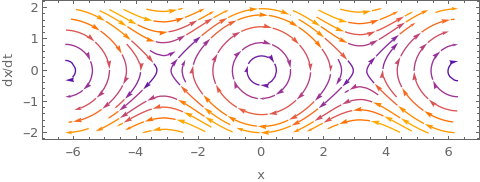
\includegraphics[width=0.7\linewidth]{2_pendulumstream}
	\caption{Phase curves of planar pendulum}
	\label{fig:2pendulumstream}
\end{figure}

\item (19) Draw the phase curves for the "equation of a pendulum on a rotating axis": $\ddot{x} = -\sin x + M$
Solution: See figure \ref{fig:2pendulumstreamrot}.
\begin{figure}
	\centering
	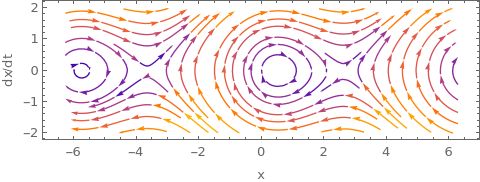
\includegraphics[width=0.7\linewidth]{2_pendulumstreamrot}
	\caption{Phase curves of rotating pendulum}
	\label{fig:2pendulumstreamrot}
\end{figure}
\item (19) Find the tangent lines to the branches of the critical level corresponding to maximal potential energy $E = U(\xi)$ (Figure \ref{fig:2critical}).\par
% TODO: \usepackage{graphicx} required
\begin{figure}
	\centering
	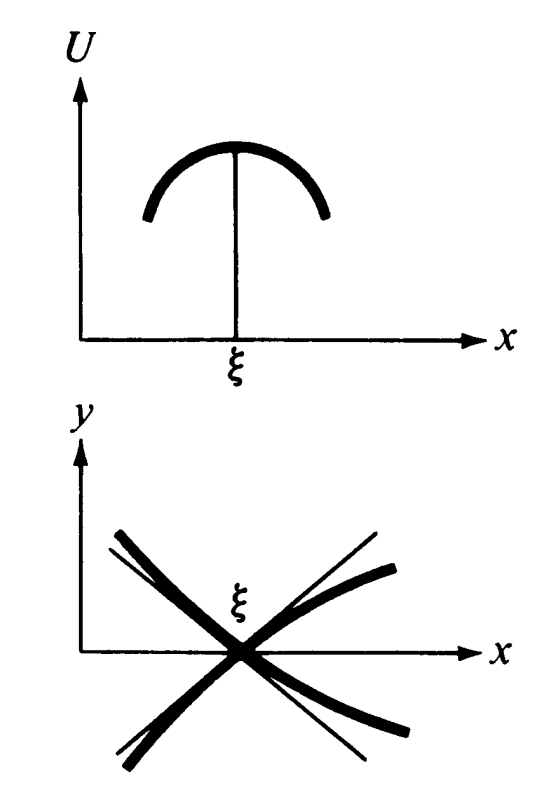
\includegraphics[width=0.5\linewidth]{2_critical}
	\caption{Critical energy level lines}
	\label{fig:2critical}
\end{figure}
Solution:  From the first problem in this chapter, we have \begin{equation}\label{key}
		\frac{y^2}{2} +U(x) = \frac{y_0^2}{2} + U(\xi) = U(\xi)\implies y = \pm\sqrt{2(U(\xi)-U(x))}
\end{equation}
Expanding $U(x)$ near the equilibrium point $\xi$, $U(x) = U(\xi)+(x-\xi)U'(\xi) +(x-\xi)^2 U''(\xi)/2 +\mathcal{O}((x-\xi)^3)$, which finally gives
\begin{equation}
	y = \pm (x-\xi)\sqrt{U''(\xi)}
\end{equation}
\item (20) Let $S(E)$ be the area enclosed by the closed phase curve corresponding to the energy level $E$. Show that the period of motion along this curve is equal to $T = \mathrm{d}S/\mathrm{d}E$.\par

Solution: Let the motion have turning points $x_1, x_2$ i.e., $U(x_1) = U(x_2) = E$, with $x_1<x_2$. Then the area under the phase space curve is given by \begin{align}\label{area}
	S(E) &= \int_{x_1}^{x_2}\mathrm{d}x|\dot{x}|+\int_{x_2}^{x_1}\mathrm{d}x(-|\dot{x}|)\\
	& = 2\int_{x_1}^{x_2}\mathrm{d}x \sqrt{2(E-U(x))}
\end{align}
where the first and second terms in equation \eqref{area} represent the motion from $x_1$ to $x_2$ and the reverse motion with negative velocity from $x_2$ to $x_1$ respectively. Now
\begin{align}
	\frac{\mathrm{d}S}{\mathrm{d}E} &= 2\int_{x_1}^{x_2}\frac{\mathrm{d}x}{\sqrt{2(E-U(x))}}\\
	&= T_{x_1\rightarrow x_2} + T_{x_2 \rightarrow x_1}
\end{align}
which gives the total time period of the motion. We have used the result of problem \ref{timeprob}.\qed
\item (20) Let $E_0$ be the value of the potential function at a minimum point $\xi$. Find the period $T_0$ of small oscillations in a neighborhood of the point $\xi$, where $T_0$ = $\lim_{E\rightarrow E_0} T(E)$.\par
Solution: Taylor expand the potential $U(x)$ near the minimum point
\begin{equation}\label{key}
	U(x) = E_0 + \frac{(x-\xi)^2}{2} U''(\xi) + \mathcal{O}((x-\xi)^3)
\end{equation}
The equation of motion gives
\begin{equation}\label{eom}
	\ddot{x} = -U'(x) = -(x-\xi)U''(\xi).
\end{equation}
Let $z = x-\xi$. Equation \eqref{eom} can be written as $\ddot{z} = -z U''(\xi)$. This is the equation of a 1-D harmonic oscillator with frequency $\omega = \sqrt{U''(\xi)}$. Thus the time period of the motion is given by $T_0 = 2\pi/\sqrt{U''(\xi)}$
\item (20) Consider a periodic motion along the closed phase curve corresponding to the energy level $E$. Is it stable in the sense of Liapunov?\par
Solution: An equilibrium point $\xi$ is said to be Liapunov stable if $\forall \epsilon>0, \exists$ $\delta(\epsilon)>0$ such that if $|x(0)-\xi|<\delta(\epsilon)$ then $|x(t)-\xi|<\epsilon$ $\forall t>0$. Simply put, we must be able to confine the motion to an arbitrarily small region of configuration space around $\xi$ by starting the motion sufficiently close to $\xi$. However, for a given periodic motion with turning points $x_1<\xi<x_2$, this is not possible for any $\epsilon<\min(\xi-x_1, x_2-\xi)$, as $|x(t)-\xi|$ will exceed this value at some point of the periodic orbit. Thus the motion is not Liapunov stable.
\item (21) Show that the system with potential energy $U = - x^4$ does not define a phase flow.\par
Solution: In order for the motion in a potential to constitute a phase flow, it must be possible to extend the solution to the entire time axis. If the motion reaches infinity in a finite amount of time, then the group properties given in the text are destroyed and thus the the motion will not define a phase flow. We now calculate the time period of motion to infinity in this potential. \par
There are two cases: $E>0$ and $E<0$. For $E<0$, let the particle have initial condition $x(0) = x_0$, $\dot{x}(0) = 0$. Its energy is given by $E = U(x_0)$. The time period for motion up to a point $x_1$ is given by (\ref{timeprob})\begin{align}\label{key}
	T &= \int_{x_0}^{x_1}\frac{\mathrm{d}x}{\sqrt{2(E-U(x))}}\\
	&\int_{x_0}^{x_1}\frac{\mathrm{d}x}{\sqrt{2(x^4-x_0^4)}}\\
\end{align}
Let $y^4 = x^4/x_0^4>0$  and let $x_1\rightarrow\infty$. Then 
\begin{equation}
	T_{\infty} = \frac{1}{\sqrt{2}x_0}\int_{1}^\infty\frac{\mathrm{d}y}{\sqrt{y^4-1}} = \frac{1}{2x_0} K\bigg(\frac{1}{\sqrt{2}}\bigg)\sim \frac{1.043}{x_0} ,
\end{equation}
where $K$ is the complete elliptic integral of the first kind (see Gradshteyn and Ryzhik - Table of Integrals, Series, and Products 7th ed.(GR) 3.166-17). For $E>0$, let $x(0) = x_0$, $\dot{x}(0) = v_0$. Its energy is given by $E = m v_0^2/2 + U(x_0)$\begin{equation}\label{key}
	T = \int_{x_0}^{x_1}\frac{\mathrm{d}x}{\sqrt{2(mv_0^2/2+x^4-x_0^4)}}.
\end{equation}
Let $z^4 = x^4/(mv_0^2/2-x_0^4)>0$ and let $x_1\rightarrow\infty$. Then 
\begin{equation}
	T_{\infty} = \frac{1}{\sqrt{2(mv_0^2/2-x_0^4)}}\int_{z_0}^\infty\frac{\mathrm{d}z}{\sqrt{z^4+1}} = \frac{1}{\sqrt{2(mv_0^2/2-x_0^4)}} F\bigg(\alpha, \frac{1}{\sqrt{2}}\bigg),
\end{equation}
where $z_0 = x_0^4/(mv_0^2/2-x_0^4)$, $F$ is the incomplete elliptic integral of first kind (GR-3.166-1) and $\alpha = (z_0^2-1)/(z_0^2+1)$.
Thus, we see that in the quartic potential, the particle reaches infinity at a finite time, and thus one cannot define a one-parameter group of diffeomorphisms. \qed
\item Show that if the potential energy is positive, then there is a phase flow.\par
Solution: Let $U(x)>0$. For bound orbits, the motion is periodic and thus can be extended to the entire time axis. For unbound orbits, let at $t=0$, $x(0) = x_0$, $\dot{x}(0)= 0$, so that the energy $E = U(x_0)>0$. The time to reach some $x_1$ is given by
\begin{equation}
	T = \int_{x_0}^{x_1}\frac{\mathrm{d}x}{\sqrt{2(U(x_0)-U(x))}}>\int_{x_0}^{x_1}\frac{\mathrm{d}x}{\sqrt{2U(x_0)}} = \frac{x_1-x_0}{\sqrt{2U(x_0)}}
\end{equation}
where we have used the fact that $U$ is positive and the orbit is unbound. Thus we see that the time period is bounded below by a linear function of $x$, and thus, for ever finite $t$, the motion in $x$ is finite, and thus the motion can be extended to the whole time axis. Thus we can define a phase flow. 
\item  Draw the image of the circ1e $x^2 + (y - 1)^2 < 1/4$ under the action of the transformation of the phase flow for the equations (a) of the "inverse pendulum," $\ddot{x} = x$ and (b) of the "nonlinear pendulum," $\ddot{x} = -\sin x$.\par
Solution: The stable equilibrium points and seperatrix can easily be inferred by observing the potential. We will derive the general solutions for the trajectories here, which can be plotted using any graphing software (DESMOS, Mathematica, etc).\par
\begin{enumerate}
	\item The general solution to the ODE can be seen to be 
\begin{align}\label{key}
	x(t) &= a e^t + b e^{-t}\\
	y(t) &= a e^t - b e^{-t}.
\end{align}
Using initial conditions $y(0) = y_0$, $x(0) = x_0$, we get
\begin{align}\label{key}
	x(t) &=\frac{x_0+y_0}{2}e^t + \frac{x_0-y_0}{2} e^{-t}\\
	y(t) &= \frac{x_0+y_0}{2} e^t - \frac{x_0-y_0}{2} e^{-t}.
\end{align}
This can be inverted easily by using $(x,y)$ as the initial conditions and evolving the system to $-t$. This gives
\begin{align}\label{key}
	x_0 &=\frac{x+y}{2}e^{-t} + \frac{x-y}{2} e^{t}\\
	y_0 &= \frac{x+y}{2} e^{-t} - \frac{x-y}{2} e^{t}.
\end{align}
One can now plot the region in the $(x,y)$ plane at time $t$ corresponding to $(x_0,y_0)$ lying in the original circle at $t=0$. They are ellipses as seen in figure \ref{invp}.
\begin{figure}[!h]
	\centering
	\subfigure[$t = 0$]{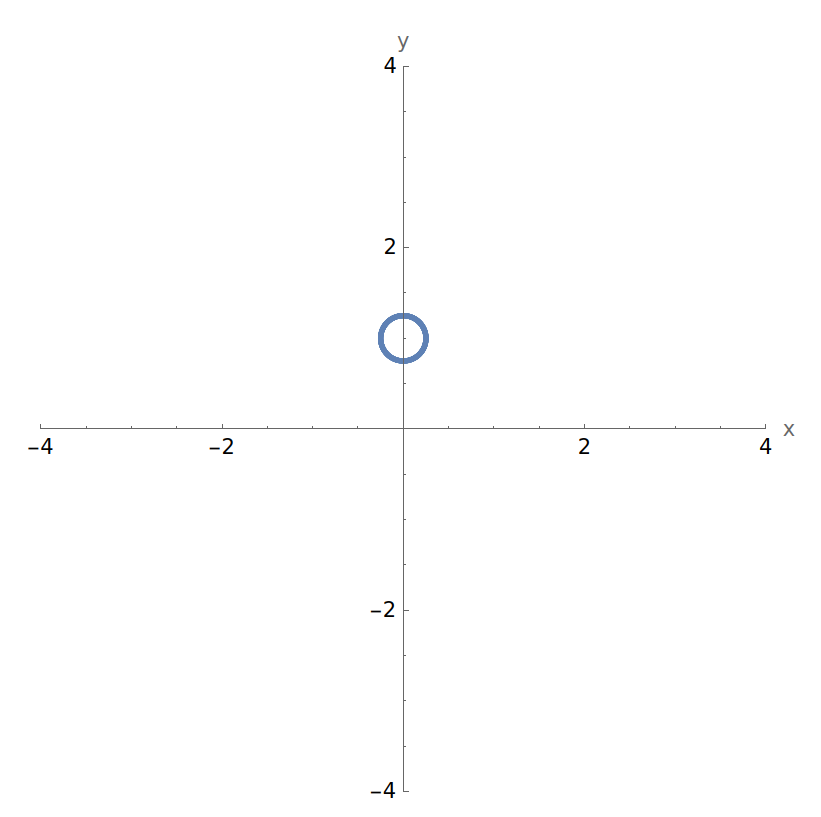
\includegraphics[width=.3\textwidth]{2_invpendulum}}
	\subfigure[$t = 0.3$]{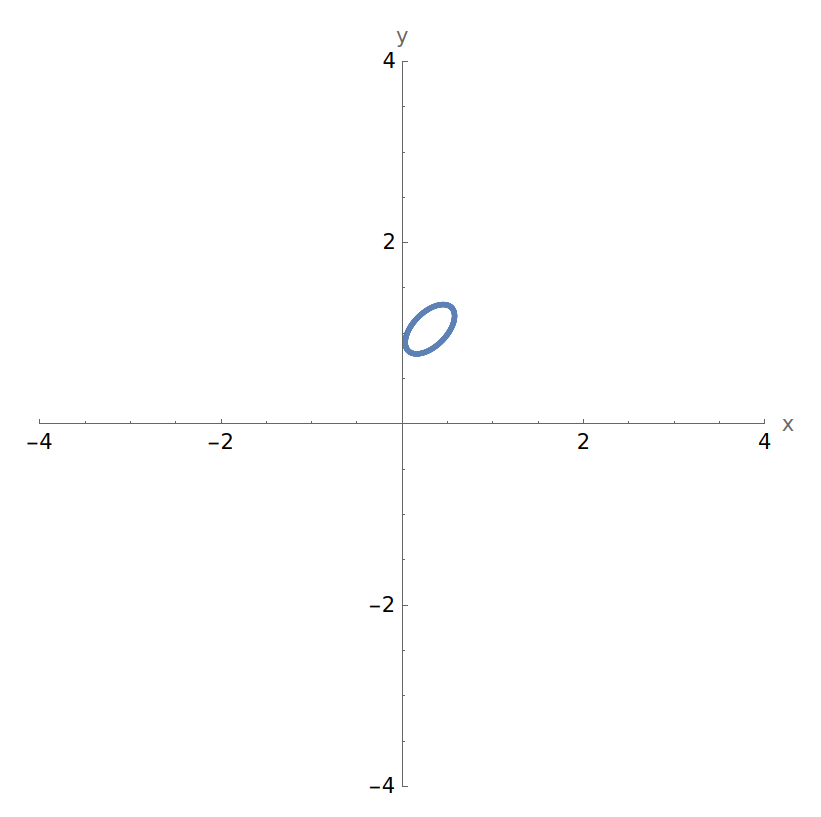
\includegraphics[width=.3\textwidth]{2_invpendulum1}}
	\subfigure[$t = 1$]{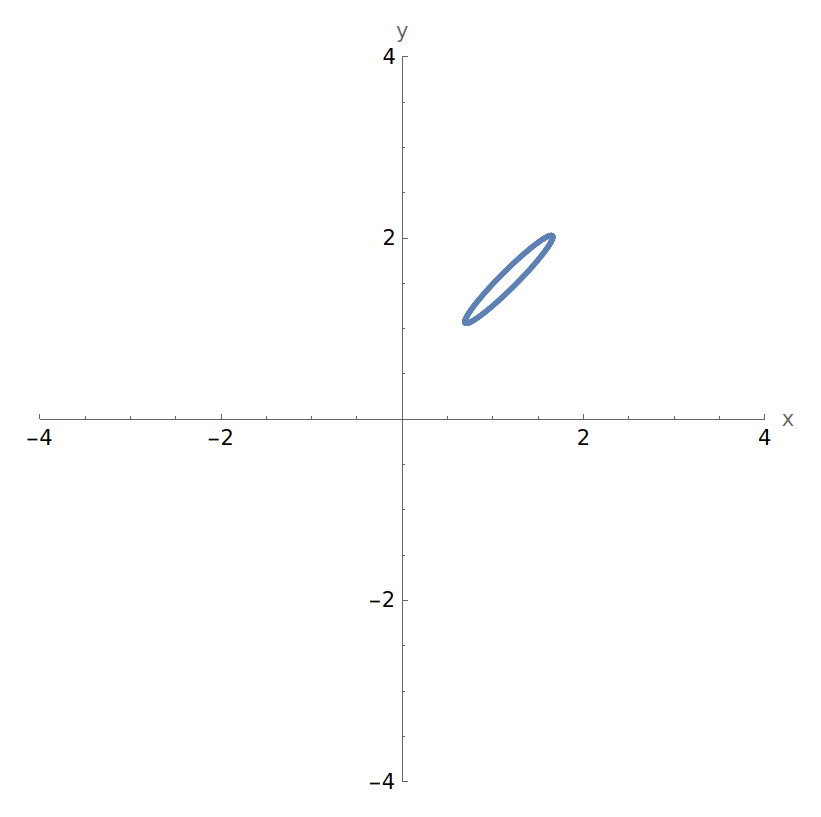
\includegraphics[width=.3\textwidth]{2_invpendulum2}}
	
	\caption{Phase plot for the inverse pendulum. The points lying on the boundary of the initial circle and subsequent motion are shown in blue.}
	\label{invp}
\end{figure}
\item This system is a lot more involved and uses elliptic integrals. The results and definitions used here may be found in GR-8.1. The ODE for $x$ can be written as 
\begin{align}
	y\mathrm{d}y & = -\sin x \mathrm{d}x\\
	y^2-y_0^2 &= 2(\cos x-\cos x_0)\label{yeqnl}\\
	y & = \sqrt{y_0^2 + 4(\sin ^2 (x_0/2)-\sin ^2 (x/2))}\\
	\mathrm{d}t & = \frac{\mathrm{d}x}{\sqrt{y_0^2 + 4(\sin ^2 (x_0/2)-\sin ^2 (x/2))}}\\
	t& = \int_{x_0}^{x}\frac{\mathrm{d}x}{2\sqrt{k_0^2-\sin^2(x/2)}},
\end{align}
where we have used standard trigonometric formulae and defined $k_0^2 \equiv y_0^2/4 + \sin^2(x_0/2)$. Define the variable $z$ such that $\sin z = \sin(x/2)/k_0$. Carrying out the change of variables, it is easy to see that
\begin{align}
	t & = \int_{z_0}^{z}\frac{\mathrm{d}z}{\sqrt{1-k_0^2\sin^2(z)}}\\
	&= F(z,k_0) - F(z_0,k_0),
\end{align}
where $ \sin z_0 = \sin(x_0/2)/k $. To invert this equation, we use the definition of the Jacobi elliptical integrals (see GR-8.14)\begin{align}\label{key}
	u &\equiv \int_0^{\mathrm{am} (u,k)}\frac{\mathrm{d}\alpha}{1-k^2\sin^2\alpha}\\
	&\equiv \int_0^{\mathrm{sn}(u,k)}\frac{\mathrm{d}t}{\sqrt{(1-t^2)(1-k^2t^2)}}
\end{align}
We thus get,\begin{align}\label{key}
	z &= \mathrm{am}(t + F(z_0,k_0),k_0)\\
	\sin z & = 	\mathrm{sn}(t + F(z_0,k_0),k_0)\\
	x(t)& = 2\arcsin(k_0 \cdot \mathrm{sn}(t + F(z_0,k_0),k_0)).
\end{align}
Now, using equation \eqref{yeqnl}, we get
\begin{align}
	y(t) &= 2\sqrt{k_0^2 - k_0^2 \mathrm{sn}^2(t + F(z_0,k_0),k_0)}\\
	& = 2 k_0 \cdot\mathrm{cn}(t + F(z_0,k_0),k_0).
\end{align}
Similar to the previous part, one can obtain the initial conditions $(x_0,y_0)$ as a function of $(x(t),y(t))$
\begin{align}
	x_0 &= 2\arcsin(k\cdot\mathrm{sn}(-t+F(z,k),k))\\
	y_0 &= 2k\cdot\mathrm{cn}(-t + F(z,k),k).
\end{align}
The circle condition may now be enforced on the initial condition which then leads to a constraint on the coordinates at later times. Qualitatively, all points trace an elliptical trajectory, with the point starting from $(0,3/4)$ having the smallest size and the point starting from $(5/4,0)$ being the largest, and all other points lying in-between. There is unstable equilibrium at $x = \pm \pi$ and a stable equilibrium at $x=0$. Any point with energy higher than the maximum value of the potential, 1, is unbound. At $x = 0$, points starting with $y>2$ are unbound. The curves starting from $y =\pm2$ and $x = 0$ form the seperatrix. As the motion proceeds, the circle is smeared more and more in phase space (phase mixing). The phase plot is shown in figure \ref{FIGURE LABEL}.
\begin{figure}[!h]
	\centering
	\subfigure[$t = 0$]{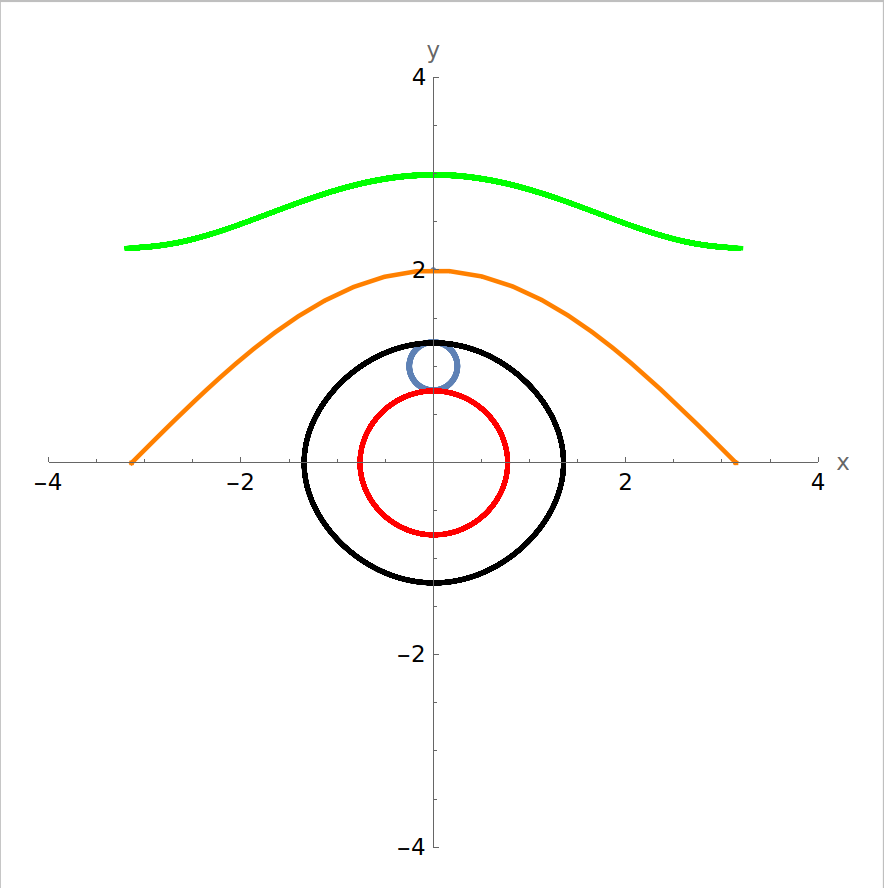
\includegraphics[width=.3\textwidth]{2_nlpendulum1}}
	\subfigure[$t = 26$]{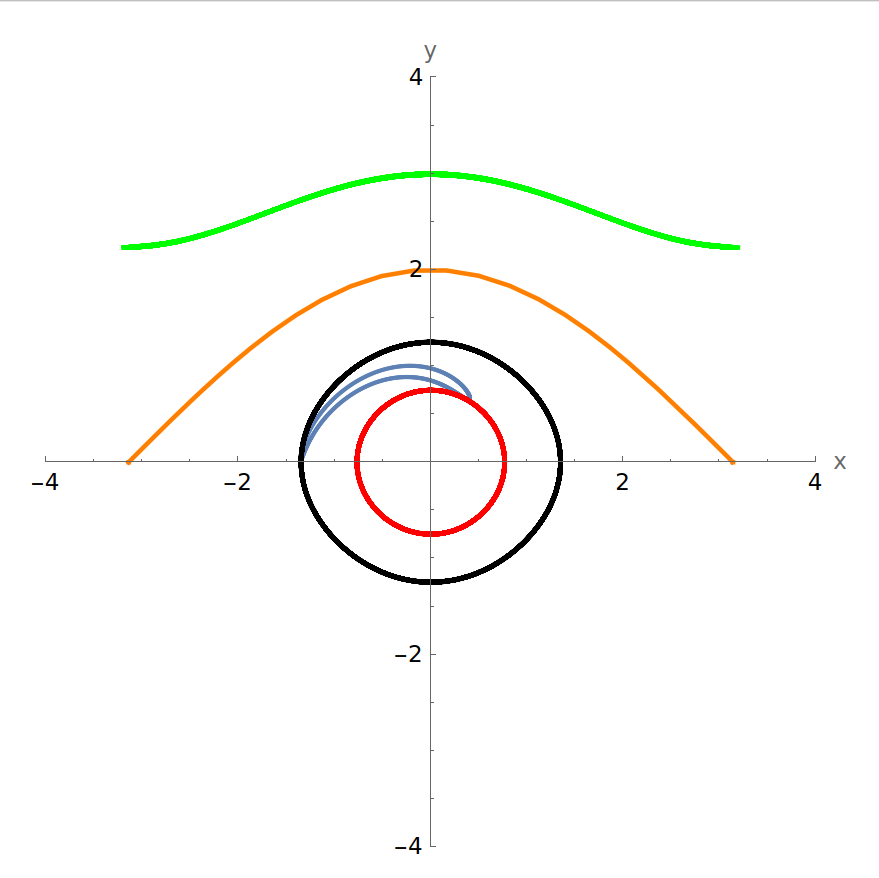
\includegraphics[width=.3\textwidth]{2_nlpendulum2}}
	\subfigure[$t = 50$]{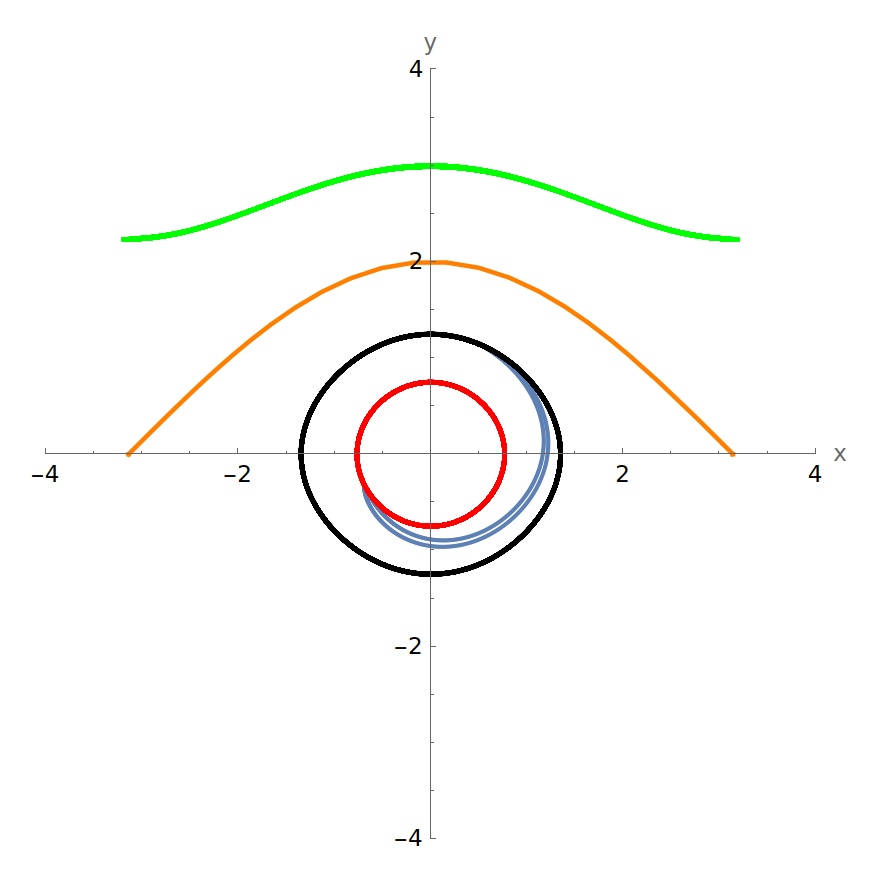
\includegraphics[width=.3\textwidth]{2_nlpendulum}}
	
	\caption{Phase plot for the non-linear pendulum. The inner and outer ellipses bounding ellipses are shown in red and black. The points lying on the boundary of the initial circle and subsequent motion are shown in blue. The seperatrix is shown in orange, and an unbound orbit is shown in green.}
	\label{FIGURE LABEL}
\end{figure}

\end{enumerate}
\end{enumerate}
